\documentclass{article}
%\usepackage{fullpage}
\usepackage{graphicx, comment, color, url}
\usepackage[round]{natbib} 
\usepackage{booktabs}
\usepackage{subfigure}
%\usepackage[small,compact]{titlesec} % saves space
\usepackage[margin=1in]{geometry}

\title{Ethics case study\\Summer Institute in Computational Social Science\footnotemark[1]}
\author{Matthew J. Salganik and Simone Zhang}
\date{June 17, 2019}

\begin{document}
\maketitle
\renewcommand{\thefootnote}{\fnsymbol{footnote}}
\thispagestyle{empty}
\footnotetext[1]{We thank Don Green for advice that helped improve this activity.  This activity is based on a similar activity in Chapter 6 of~\citet{salganik_bit_2018} and based on an activity from SICSS 2017 (created by Matthew Salganik and Yo-Yo Chen) and SICSS 2018 (created by Matthew Salganik and Janet Xu).} 
\renewcommand{\thefootnote}{\arabic{footnote}}

In August 2006, about 10 days prior to an election, 20,000 people living in Michigan received something surprising in the mail.  They received a mailer that asked ``WHAT IF YOUR NEIGHBORS KNEW WHETHER YOU VOTED?'' (caps in original). Unlike the usual mailers that campaigns and political organizations send to potential voters, this one featured a table showing the actual voting behavior of the recipient's neighbors in previous elections (Fig.~\ref{fig:gerber_social_2008_neighbors}). 

This mailer was part of a research experiment on voting behavior.  One-time mailings typically increase voter turnout by about one percentage point, but this particular one increased turnout by 8.1 percentage points, the largest effect seen up to that point~\citep{gerber_social_2008}.  The effect was so large that a political operative named Hal Malchow offered the researcher \$100,000 not to publish the result of the experiment, presumably so that Malchow could make use of this information himself~\citep[p. 304]{issenberg_victory_2012}.  But, the researchers did ultimately publish the paper in 2008 in the \textit{American Political Science Review.} The abstract of the paper explains the scientific motivations for the study:

\begin{quote}
``Voter turnout theories based on rational self-interested behavior generally fail to predict significant turnout unless they account for the utility that citizens receive from performing their civic duty. We distinguish between two aspects of this type of utility, intrinsic satisfaction from behaving in accordance with a norm and extrinsic incentives to comply, and test the effects of priming intrinsic motives and applying varying degrees of extrinsic pressure. A large-scale field experiment involving several hundred thousand registered voters used a series of mailings to gauge these effects. Substantially higher turnout was observed among those who received mailings promising to publicize their turnout to their household or their neighbors. These findings demonstrate the profound importance of social pressure as an inducement to political participation.''
\end{quote}
 
In addition to the 20,000 mailers that asked ``WHAT IF YOUR NEIGHBORS KNEW WHETHER YOU VOTED?,'' the researchers also sent 60,000 other mailers with three slightly different designs (Fig.~\ref{fig:gerber_social_2008_civicduty},~\ref{fig:gerber_social_2008_hawthorne}, and \ref{fig:gerber_social_2008_self}).  When you carefully inspect the mailers you may notice that the researchers' names do not appear on them.  Rather, the return address is to Practical Political Consulting.  In the acknowledgments section of the paper, the authors explain: ``Special thanks go to Mark Grebner of Practical Political Consulting, who designed and administered the mail program studied here.''  The acknowledgments section of the paper also makes clear that this study was approved be the Human Subjects Committee (i.e., Institutional Review Board) at the researchers' university.
 
Some people who received these mailers were not happy.  In fact,~\citet[p. 198]{issenberg_victory_2012} reports that ``Grebner [the director of Practical Political Consulting] was never able to calculate how many people took the trouble to complain by phone, because his office answering machine filled so quickly that new callers were unable to leave a message.'' Grebner further suggested that the backlash could have been even larger if they had scaled up the experiment.  He said to Alan Gerber, one of the researchers, ``Alan if we had spent five hundred thousand dollars and covered the whole state you and I would be living with Salman Rushdie.''~\citep[p. 200]{issenberg_victory_2012}.\footnote{Salman Rushdie is a British Indian author. He was placed under police protection when his fourth novel, \textit{The Satanic Verses}, provoked protests and led the Supreme Leader of Iran to issue a fatwa ordering his assassination.}
 
This particular case is great for a discussion because it is interesting and important research, and it touches on many of the ethical issues that arise in computational social science in unexpected ways.  It is also a great case because there are no easy answers.  Please discuss these questions in your group:

\begin{enumerate}
\item Before you proceed, please quickly read the paper: \url{https://doi.org/10.1017/S000305540808009X}.  If this were a real ethical discussion---not an activity---you would need to be very familiar with the research itself.
\item Assess the ethical issues raised by this study.  Please draw on any framework, principles, or ideas that you think are appropriate.
\item Given your assessment, what approaches would you take to address the ethical issues that this study raises?  These approaches could be related to the design, testing, or publishing of the study.
\item Would it impact your answer to the questions above if Mark Grebner was already sending out similar mailings at this time?  More generally, how should researchers think about evaluating existing interventions created by practitioners?
\end{enumerate}
 

\begin{figure}
\centering
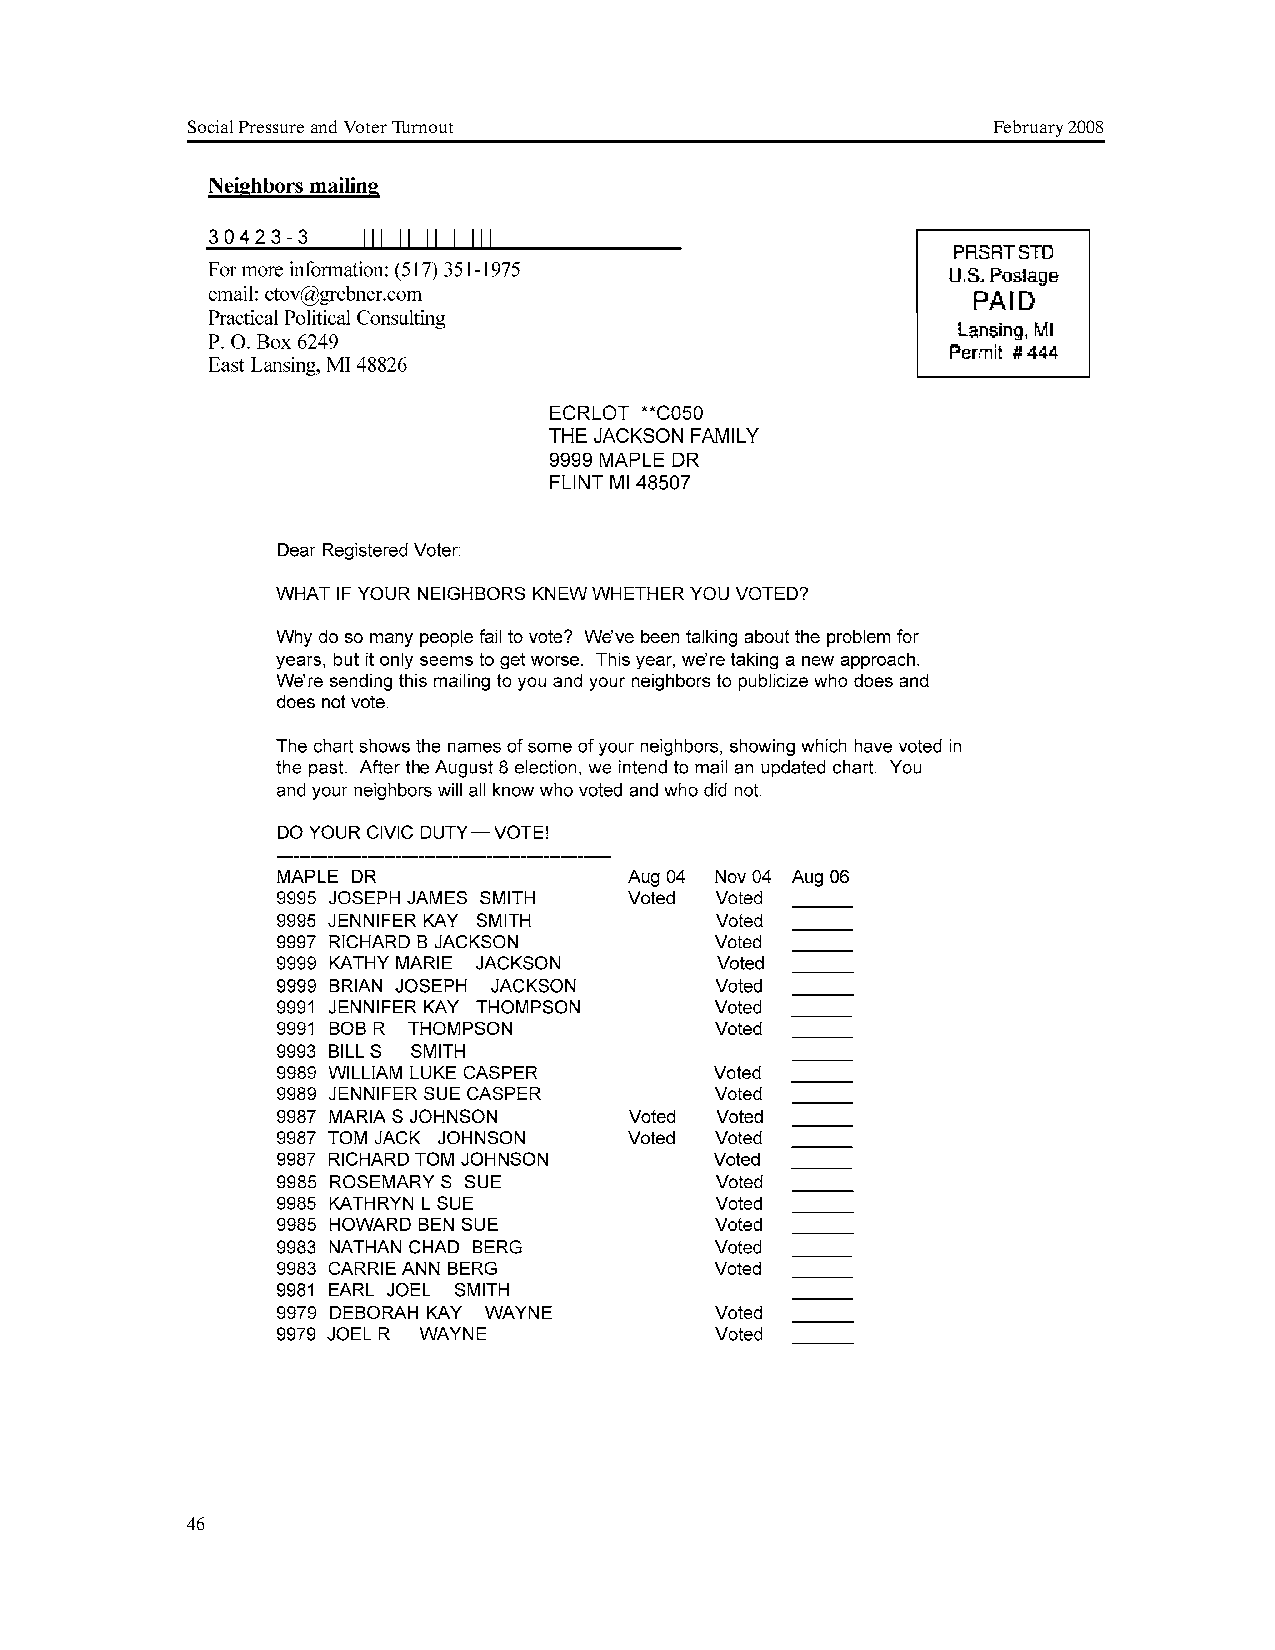
\includegraphics[width=\textwidth]{figures/gerber_social_2008_neighbors}
\caption{Neighbor mailer from~\citet{gerber_social_2008}.}
\label{fig:gerber_social_2008_neighbors}
\end{figure}

\begin{figure}
\centering
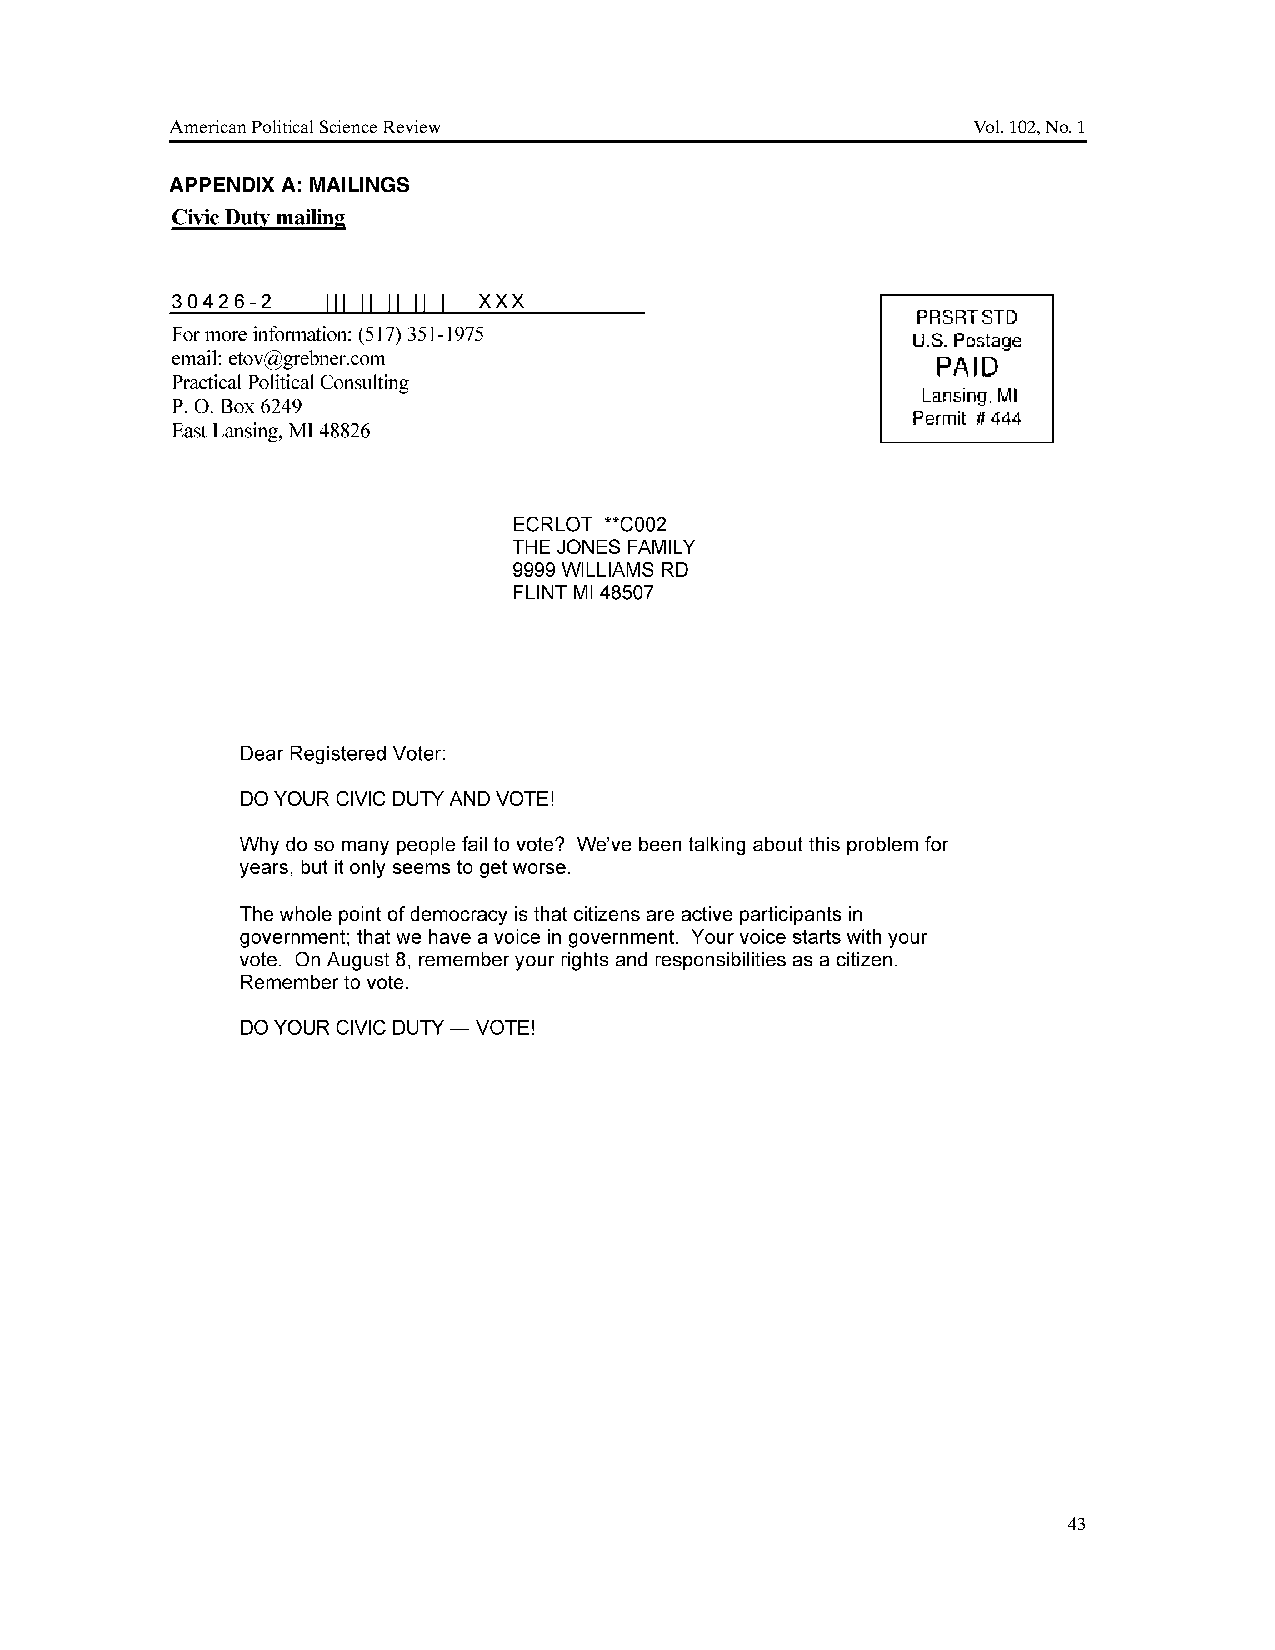
\includegraphics[width=\textwidth]{figures/gerber_social_2008_civicduty}
\caption{Civic duty mailer from~\citet{gerber_social_2008}.}
\label{fig:gerber_social_2008_civicduty}
\end{figure}

\begin{figure}
\centering
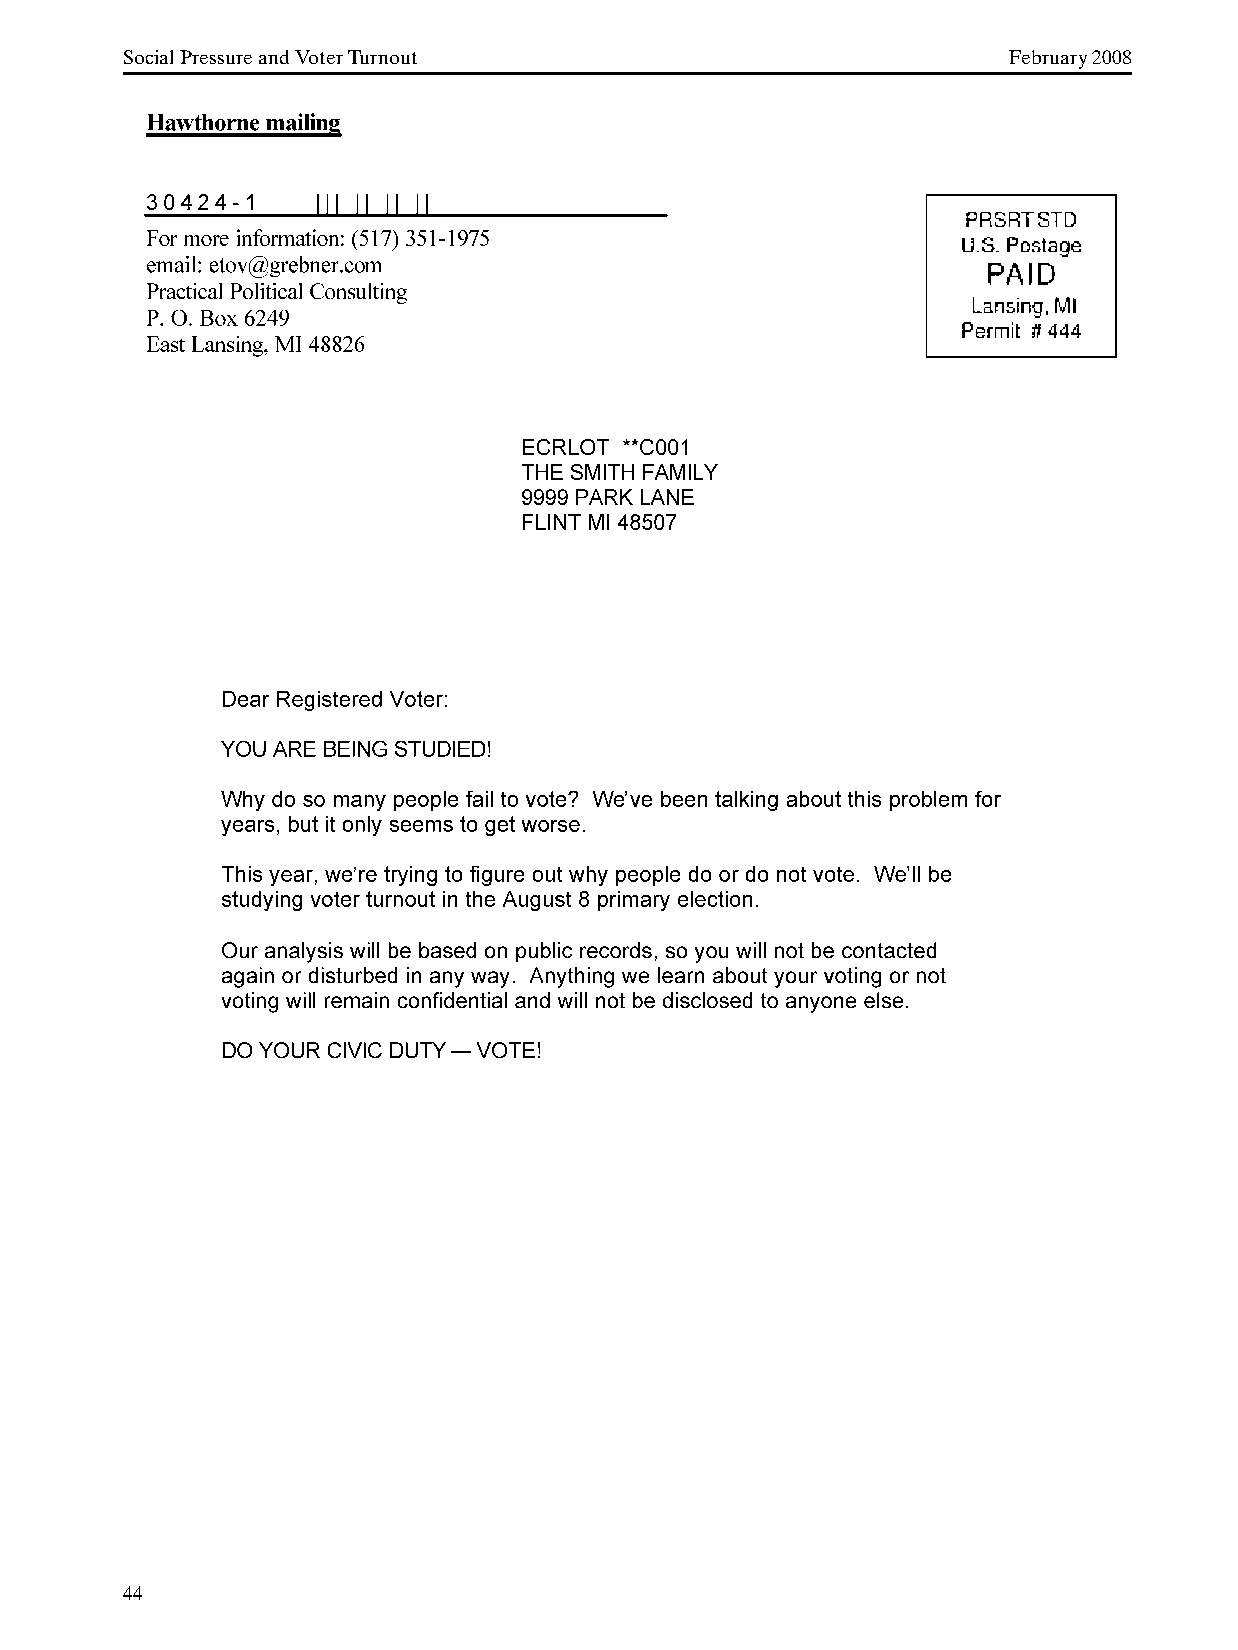
\includegraphics[width=\textwidth]{figures/gerber_social_2008_hawthorne}
\caption{Hawthorne mailer from~\citet{gerber_social_2008}.}
\label{fig:gerber_social_2008_hawthorne}
\end{figure}

\begin{figure}
\centering
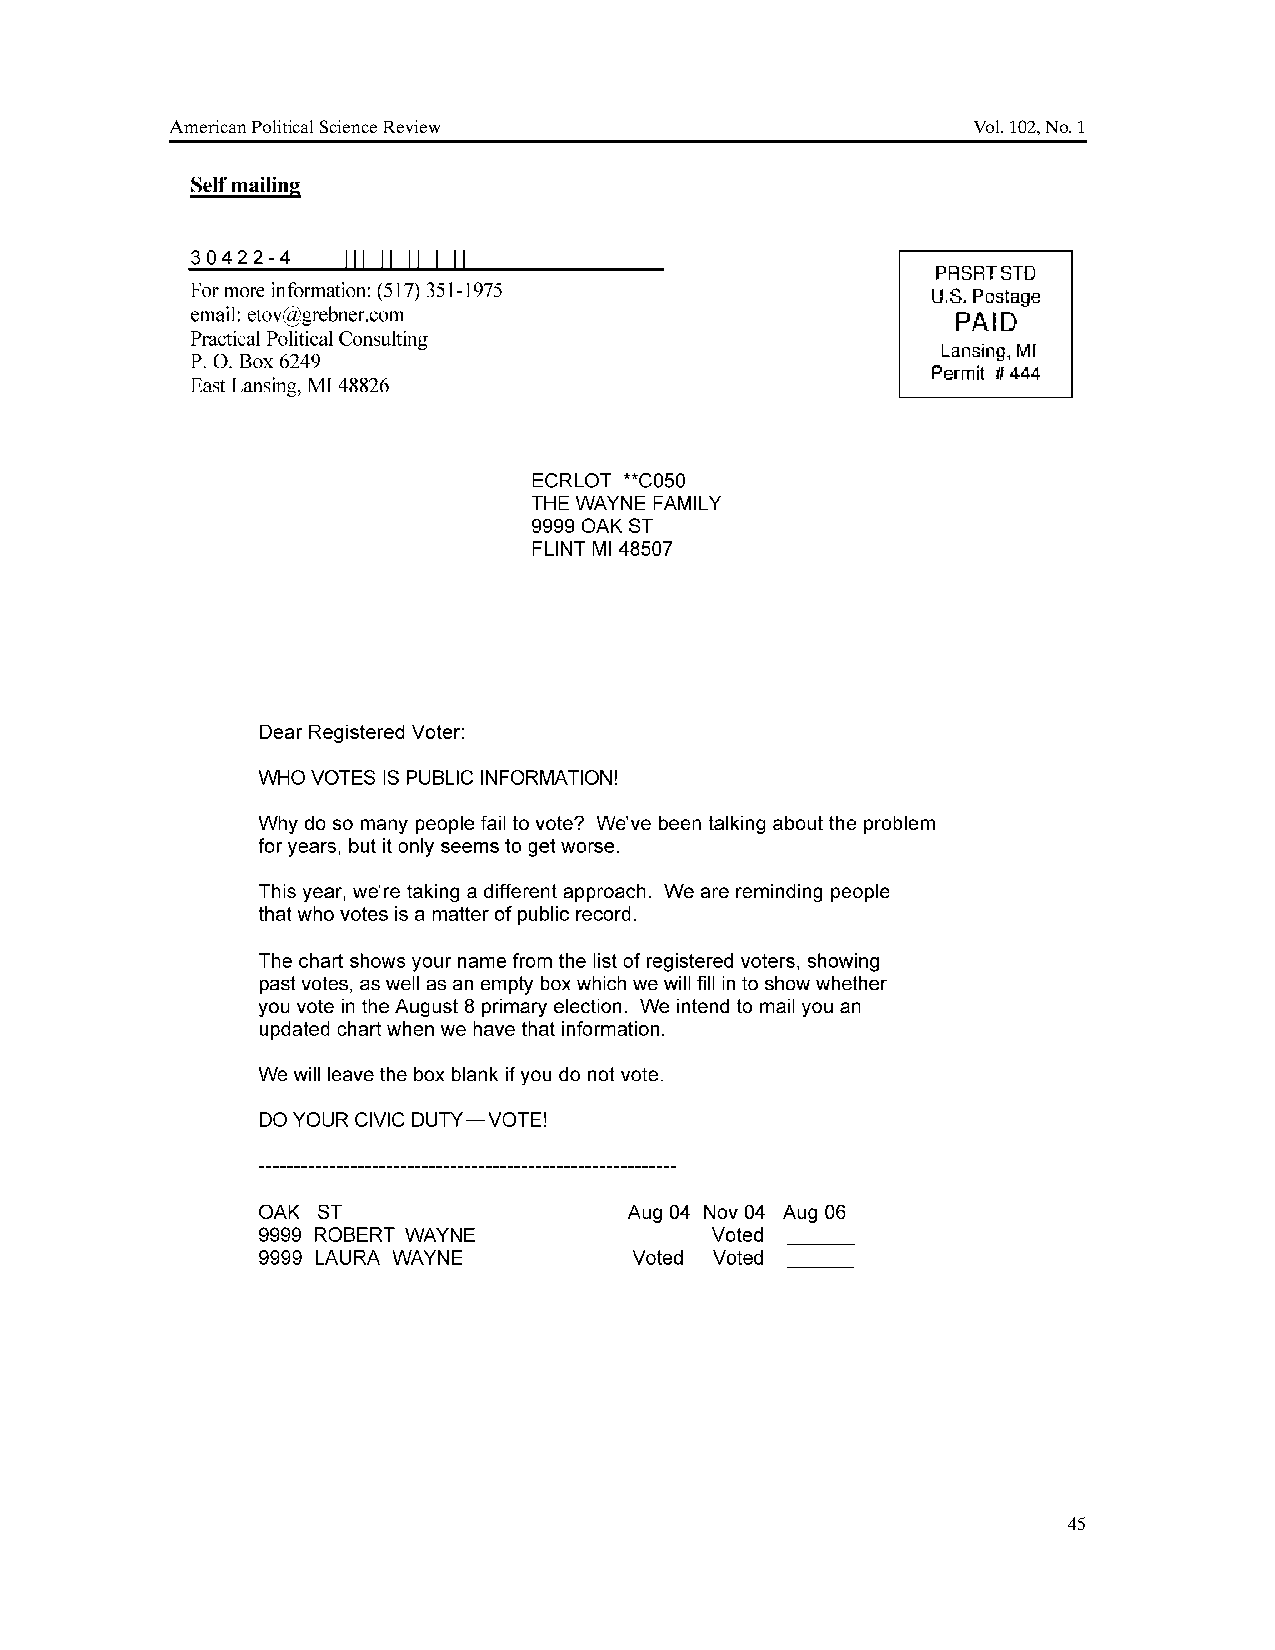
\includegraphics[width=\textwidth]{figures/gerber_social_2008_self}
\caption{Self mailer from~\citet{gerber_social_2008}.}
\label{fig:gerber_social_2008_self}
\end{figure} 
 
 
\bibliographystyle{apalike} 
\bibliography{ethics}
\end{document}
